\documentclass[12pt, a4paper]{article}
\usepackage{float}
\usepackage{geometry}
\usepackage{graphicx}
\geometry{left=20mm,right=20mm,top=20mm,bottom=20mm}
\linespread{1.1}
\begin{document}
\begin{titlepage}
\begin{center}
%\huge{\bfseries{SHRM ASSIGNMENT}}\\
%[5cm]
\huge{\textsc{POST MERGER ANALYSIS OF CUSTOMER SATISFACTION AND LOYALTY , A STUDY ON RECENT MERGER OF ASSOCIATE BANKS OF A POPULAR BANK WITH ITSELF}}\\
\end{center}
\begin{flushright}
\emph{\large{Submitted by,}}\\
\large{Adhithyan V}\\
\large{(2016201002)}
\end{flushright}
\end{titlepage}

\noindent\makebox[\linewidth]{\rule{\paperwidth}{0.4pt}}
\section*{PROBLEM STATEMENT}
\par A satisfied customer remains loyal and spreads positive word of mouth. Mergers and acquisitions often focus on financial aspects but rarely consider the customer facet of mergers. Studies show that 2/3 rd of mergers fail due to dissatisfied customers.A dissatisfied customer also switches the brand.Merger process are often done without considering the customers. Studies have found that more than half of all mergers fail to deliver the intended improvement in stakeholder value and that customer defections contribute to that high failure rate (Hitt et al., 2007). Thus, a harmonious integration of the beliefs and values of a merging firm and the ability to integrate organisational cultures is more important to success than the financial or strategic factors (Majidid, 2007). Customer switching also increases post merger. This study aims to find out loyalty and customer satisfaction post merger considering various factors such as demographics, brand image, psychological breach of contract etc taking the recent merger of associate banks of SBI with itself as a case study. 

\section*{NEED FOR THE PROJECT}
Most of the merger effectiveness are assessed based on financial performance, synergy. Rarely the studies assess the effectiveness of merger from customer perspective.The success of merger depends not only on financial aspects but also creating value for its stakeholders. There has been lot of failed mergers because most of the mergers didn't consider human aspects of merger.  This study is important to find out level of service changes in banks post merger and their impact on customer satisfaction and loyalty due to service changes and psychological breach of contract. \emph{A psychological contract breach refers to subjective perception that other party has failed to adequately fulfill promised obligations.} This study will also be useful to assess the effectiveness of merger from customer point of view.
\section*{OBJECTIVES}
\subsection*{Primary Objective}
\begin{itemize}
\item To find the customer satisfaction and loyalty post merger.
\end{itemize}
\subsection*{Secondary objectives}
\begin{itemize}
\item To study about change resistance.
\item To find out various issues faced by customer post merger
\item To find out the benefits of mergers from customer perspective.
\end{itemize}

\section*{SCOPE OF THE STUDY}
The associate banks of State Bank of India (SBI) that merged with it recently are State Bank of Bikaner and Jaipur (SBBJ), State Bank of Mysore (SBM), State Bank of Travancore (SBT),  State Bank of Hyderabad (SBH),  State Bank of Patiala (SBP).
This study does not cover SBBJ and SBP. The remaining associate banks located in Pollachi, Salem and Chennai will be included in the study. 

\section*{RESEARCH MODEL}
\begin{figure}[H]
\centering
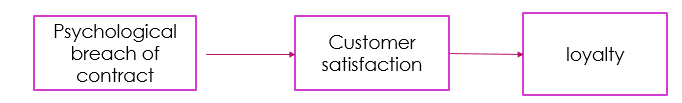
\includegraphics[scale=1]{model.png}
\end{figure}
\begin{itemize}
\item Psychological breach of contract has negative influence on customer satisfaction.
\item Customer satisfaction has positive impact on customer loyalty.
\end{itemize}
\section*{LITERATURE REVIEW}
\begin{itemize}
\item Trust and satisfaction increases customers intention to reuse the product. Psychological contract violation affects customer satisfaction and their intention to use the product. \emph{(Psychological contract violation and customer intention to reuse online retailers - Neeru Malhotra a, Sunil Sahadev b, Keyoor Purani ., 2017)}
\item Customer often compare the pre and post merger service changes. Nostalgia plays an important role in this. \emph{(Effect of nostalgia on customer loyalty to Brand Post-merger / acquistions – Ana Carolina Toledo, Evandro Luiz Lopes., 2016)}
\item Various factors like satisfaction, trustworthiness, image and relationship affect customer loyalty and firms should maintain them at any cost – \emph{( Affecting customer loyalty: Do different factors have various influences in different loyalty levels – Andres kussik  - 2007)}
\end{itemize}
\section*{RESEARCH GAP}
This study has not been conducted before. This is the first such attempt to assess merger effectiveness from customer point of view. Psychological breach of contract in banking sector from customer perspective have not been studied before.  Studies on this topic has been done on e-Commerce.

\end{document}